
\documentclass[article]{llncs}
%
\usepackage[utf8]{inputenc}
\usepackage[spanish]{babel}
\usepackage{graphicx}
% Used for displaying a sample figure. If possible, figure files should
% be included in EPS format.
%
% If you use the hyperref package, please uncomment the following line
% to display URLs in blue roman font according to Springer's eBook style:
% \renewcommand\UrlFont{\color{blue}\rmfamily}


\begin{document}
%
\title{Detecci\'on de Instalaciones con Machine Learning}
%
%\titlerunning{Abbreviated paper title}
% If the paper title is too long for the running head, you can set
% an abbreviated paper title here
%
\author{Jes\'us Santos Capote, Kenny Villalobos Morales, Jorge Soler Gonz\'alez, Abraham Gonz\'alez Rivero, 
Rainel Fern\'andez Abreu, Eduardo Garc\'ia Maleta}
%
\institute{Facultad de Matemática y Computación, Universidad de La Habana, La Habana, Cuba }
%
\maketitle              % typeset the header of the contribution
%

\keywords{Detección de Objetos \and Clasificación de Im\'agenes \and Machine Learning \and Pytorch \and Keras \and Tensorflow \and Faster-RCNN}


\section{Intoducci\'on}
El uso de imágenes satelitales ha permitido avances significativos en la identificación y caracterización de diferentes 
tipos de construcciones, lo cual puede ser de gran utilidad en diversas áreas como la planificación urbana, la gestión de 
recursos naturales y la seguridad nacional, entre otras. Los autores proponen cuatro modelos, dos de clasificación de im\'agenes, 
uno de detección de objetos y uno segmentaci\'on con el fin de identificar en im\'agenes satelitales edificaciones con una topolog\'ia espec\'ifica.

\section{Estado del Arte}

\subsection{Aprendizaje no Supervisado}

El problema de detección y clasificación de imágenes satelitales puede abordarse mediante el uso de técnicas de 
aprendizaje no supervisado. El aprendizaje no supervisado implica el entrenamiento de un modelo sin la necesidad de 
etiquetas de datos previas. En lugar de eso, el modelo busca patrones y estructuras en los datos sin una guía explícita.

A continuación, se describen algunas técnicas de aprendizaje no supervisado que se pueden utilizar para abordar el 
problema de detección y clasificación de imágenes satelitales:

\subsubsection{Clustering:} Esta técnica implica agrupar los datos en grupos o clusters, donde cada cluster contiene datos similares. 
En el contexto de las imágenes satelitales, se pueden agrupar los píxeles en clusters en función de su color, textura o 
características espectrales. Los clusters resultantes pueden usarse para identificar regiones de interés en la imagen.

Los resultados de aplicar clustering a la clasificación y detección de imágenes satelitales pueden ser prometedores. 
En general, el clustering puede ayudar a identificar regiones de interés en la imagen satelital y reducir la complejidad 
de los datos. Sin embargo, es importante tener en cuenta que la calidad de los resultados depende de la calidad de los 
datos y la elección del algoritmo de clustering. Además, el clustering no proporciona información sobre las 
características específicas de los objetos en la imagen, por lo que puede ser necesario combinar el clustering con otras 
técnicas de procesamiento de imágenes para obtener una clasificación y detección más precisa.

\subsubsection{Autoencoder:} Un autoencoder es una red neuronal que se entrena para reconstruir una entrada a través de 
una capa oculta. En el contexto de las imágenes satelitales, se puede utilizar un autoencoder para extraer 
características latentes de la imagen. Las características latentes se pueden utilizar para identificar patrones y 
estructuras en la imagen que pueden ayudar en la detección y clasificación.

\subsubsection{Análisis de componentes independientes (ICA):}Esta técnica implica descomponer una señal en sus 
componentes independientes. En el contexto de las imágenes satelitales, se puede utilizar el ICA para separar las 
fuentes de la señal, como la vegetación, el agua y la tierra. Los componentes resultantes se pueden utilizar para 
identificar regiones de interés en la imagen.

\subsubsection{Análisis de componentes principales (PCA) aplicado a imágenes:} Esta técnica se utiliza para reducir la dimensión de 
las imágenes satelitales, lo que puede hacer que los algoritmos de clasificación sean más eficientes. PCA se utiliza para 
extraer las características más relevantes de las imágenes, lo que permite representarlas en un espacio de menor 
dimensionalidad. El objetivo de PCA es encontrar una transformación lineal que permita representar los datos originales 
en un nuevo espacio de menor dimensión. Esta transformación se realiza de tal manera que la primera componente principal 
capture la mayor varianza posible de los datos, la segunda componente principal capture la mayor varianza posible que 
queda después de haber eliminado la primera componente, y así sucesivamente. Las componentes principales se calculan de 
tal manera que sean ortogonales entre sí.

En el contexto de la clasificación de imágenes satelitales, se pueden utilizar las bandas de las imágenes como 
características y aplicar el algoritmo de clustering K-Means para agrupar las imágenes en diferentes categorías de 
cobertura terrestre.

Una variante del algoritmo de K-Means, llamada K-Means espectral, utiliza una representación de grafos de los datos para 
llevar a cabo el clustering. En esta variante, los píxeles de las imágenes se representan como nodos de un grafo y se 
calcula una matriz de afinidad entre ellos. Luego, se aplica el algoritmo de clustering K-Means en la matriz de afinidad 
para agrupar los píxeles en diferentes categorías de cobertura terrestre.

Otra técnica es la segmentación de imágenes, que implica dividir las imágenes en regiones homogéneas basadas en la 
similaridad de los píxeles. La segmentación se puede realizar utilizando técnicas como la segmentación por umbral, la 
segmentación basada en regiones y la segmentación basada en contornos. Luego, se pueden utilizar técnicas de clustering 
para agrupar las regiones segmentadas en diferentes categorías de cobertura terrestre.

\subsection{Artículos relacionados:} 

- Unsupervised Deep Feature Extraction
  for Remote Sensing Image Classification

  Presentan un enfoque para la extracción de características en imágenes de teledetección utilizando redes neuronales 
  convolucionales (CNN) no supervisadas.

  En lugar de utilizar etiquetas de clase para entrenar la CNN, el enfoque propuesto utiliza un algoritmo de clustering 
  no supervisado para dividir las imágenes en diferentes grupos, y luego utiliza la CNN para extraer características de 
  cada grupo de manera independiente. Estas características se utilizan posteriormente para clasificar las imágenes en 
  diferentes categorías.

  Los resultados experimentales demuestran que el enfoque propuesto puede mejorar significativamente la precisión de la 
  clasificación en comparación con otros métodos existentes. En particular, los autores compararon su enfoque con otros 
  tres métodos de clasificación de imágenes de teledetección en dos conjuntos de datos diferentes.

  En el primer conjunto de datos, que consta de imágenes del sensor remoto AVIRIS, el enfoque propuesto superó a los 
  otros métodos en términos de precisión de clasificación, alcanzando una precisión del 93,74\%. En el segundo conjunto 
  de datos, que consta de imágenes del sensor remoto HYDICE, el enfoque propuesto también superó a los otros métodos, 
  alcanzando una precisión del 93,47\%.

- Unsupervised Feature Learning in Remote Sensing

  En este artículo se propone un algoritmo de aprendizaje no supervisado de última generación al conjunto de datos xView, 
  ruidoso y extremadamente desequilibrado, para entrenar un extractor de características que se adapta a varias tareas: 
  búsqueda de similitud visual que funciona bien tanto en clases comunes como raras; identificación de valores atípicos 
  dentro de un conjunto de datos etiquetados; y aprendizaje automático de una jerarquía de clases natural.

  Las conclusiones de los autores luego de experimentar fueron:

  El aprendizaje de características no supervisado (UFL) supera significativamente a los modelos de autoencoder en la 
  tarea de clasificación de imágenes no supervisada. UFL logró una precisión del 18,3\% en el top 1 y del 54,5\% en el 
  top 5, en comparación con solo el 3,6\% y el 19,9\% para el autoencoder.

  El preentrenamiento del modelo UFL en ImageNet antes del fine-tuning en el conjunto de datos objetivo (xView) conduce 
  a una gran mejora en el rendimiento. El modelo UFL preentrenado logró una precisión del 12,9\% en el top 1 y del 47,6\% 
  en el top 5 sin ningún fine-tuning en xView.

  El fine-tuning del modelo UFL en el conjunto de datos objetivo después del preentrenamiento en ImageNet mejora aún más 
  el rendimiento. El fine-tuning aumentó la precisión del top 1 del 12,9\% al 18,3\% y la precisión del top 5 del 47,6\% 
  al 54,5\%.

  El uso de una CNN más profunda (ResNet50 frente a ResNet18) conduce a un pequeño aumento en el rendimiento para el 
  modelo UFL. Sin embargo, ResNet18 todavía logra un rendimiento bastante bueno mientras es más rápido y menos costoso 
  computacionalmente.

  El rendimiento del modelo supervisado (42,4\% en el top 1, 65,6\% en el top 5) establece un límite superior en la 
  precisión que se puede lograr sin usar información de etiqueta durante el entrenamiento. El modelo UFL logra un 
  rendimiento bastante bueno considerando que se entrena de manera completamente no supervisada, sin acceso a datos de 
  etiqueta.

  El muestreo equilibrado por clase durante el entrenamiento probablemente mejoraría el rendimiento del modelo UFL, 
  pero requiere acceso a información de etiqueta y, por lo tanto, no se utilizó. Se usó un muestreo equilibrado por 
  clase para el modelo supervisado.

- Spectral-Spatial Feature Extraction for Hyperspectral Image Classification: A Dimension Reduction and Deep Learning 
Approach

  Los autores proponen una técnica que utiliza la reducción de dimensionalidad y el aprendizaje profundo para extraer 
  características espectrales y espaciales de las imágenes hiperspectrales, con el objetivo de mejorar la precisión de 
  la clasificación.

  La técnica propuesta consta de dos etapas principales como el anterior. En la primera etapa, se utiliza el análisis 
  de componentes principales (PCA) para reducir la dimensión de las imágenes hiperspectrales. PCA se aplica a cada 
  banda espectral de la imagen, lo que permite reducir la dimensión de las imágenes mientras se mantiene la información 
  más relevante. Como resultado, se obtiene una representación de las imágenes en un espacio de menor dimensión.

  En la segunda etapa, se utiliza una red neuronal convolucional (CNN) para aprender una representación de 
  características espaciales y espectrales de las imágenes hiperspectrales. La CNN se entrena utilizando la 
  representación de las imágenes obtenida en la primera etapa, y se utiliza para clasificar las imágenes en diferentes 
  categorías.

  En el primer conjunto de datos, que consta de imágenes hiperespectrales de la Tierra, el enfoque propuesto superó a 
  los otros métodos en términos de precisión de clasificación, alcanzando una precisión del 94,03\%. Los métodos 
  comparativos incluidos en este conjunto de datos fueron el análisis discriminante lineal (LDA), el análisis de 
  discriminante cuadrático (QDA), la máquina de vectores de soporte (SVM) y el enfoque basado en PCA.

  En el segundo conjunto de datos, que consta de imágenes hiperespectrales de cultivos, el enfoque propuesto también 
  superó a los otros métodos, alcanzando una precisión del 98,57\%. Los métodos comparativos incluidos en este conjunto 
  de datos fueron LDA, QDA, SVM y el enfoque basado en PCA.


\subsection{Aprendizaje Supervisado}

Una de las aplicaciones más comunes del aprendizaje supervisado en la detección y clasificación de objetos en imágenes 
satelitales es la detección de edificios, carreteras, cuerpos de agua y otros objetos de interés. Para entrenar un 
modelo de aprendizaje automático, se recopila una base de datos de imágenes satelitales con objetos etiquetados y se 
utiliza para entrenar el modelo. Una vez que se ha entrenado el modelo, se puede utilizar para detectar y clasificar 
objetos similares en nuevas imágenes satelitales.

El aprendizaje profundo es una técnica popular que se utiliza para la detección de objetos en 
imágenes satelitales. Los modelos de aprendizaje profundo, como las redes neuronales convolucionales (CNN), pueden 
aprender características complejas de las imágenes satelitales, lo que les permite detectar objetos con mayor precisión.

Además del aprendizaje profundo, existen otras técnicas de aprendizaje supervisado que se utilizan en la detección y 
clasificación de objetos en imágenes satelitales, como la clasificación basada en árboles de decisión, la regresión 
logística y los clasificadores de vectores de soporte.

\subsection{Articulos Relacionados}

- Detection by classification of buildings in multispectral satellite imagery

  El enfoque de los autores consiste en entrenar una Red Neuronal Convolucional (CNN) desde cero para clasificar parches de 
  imágenes multiespectrales tomadas por satélites como si pertenecieran o no a una clase de edificios. Luego se adapta 
  la red de clasificación para la detección convirtiendo las capas completamente conectadas de la red en capas 
  convolucionales, lo que permite que la red procese imágenes de cualquier resolución.

- Satellite Image Classification with Deep Learning

  Los autores proponen un ensamblado de redes neuronales convolucionales y redes neuronales adicionales que integran los 
  metadatos satelitales con las características de las imágenes. Las CNN extraer\'an un mapa de caracter\'isticas que 
  luego se convina con metadatos de las im\'agenes para alimentar una red neuronal densa que aprender\'a a clasificar el 
  objeto principal de la im\'agen. Los metadatos no se filtran pues la idea es que la red aprenda que metadato es m\'as importante 
  en la clasificaci\'on. En el momento en que los autores escribieron el art\'iculo, el sistema se encuentraba en segundo lugar en la competencia 
  TopCoder de fMoW(Functional Map of The World). Su precisión total es del 83\%, el puntaje F1 es de 0.797, y clasifica 15 de las clases con una 
  precisión del 95\% o mejor.

- Detection, Classification and Boundary Regularization of Buildings in Satellite Imagery Using Faster Edge Region 
Convolutional Neural Networks

  En este artículo, con el fin de mejorar la precisión de la detección y clasificación de edificios, los autores proponen un 
  algoritmo de Faster Edge Region Convolutional Neural Networks (FER-CNN). Este algoritmo propuesto se entrena y evalúa 
  en diferentes conjuntos de datos. Además, proponen un nuevo método para mejorar la detección de los límites de los 
  edificios detectados. Los resultados del algoritmo se comparan con los de otros métodos, como el Faster Region 
  Convolution Neural Network (Faster R-CNN) clásico con el VGG16 original y el Single-Shot Multibox Detector (SSD). Los 
  resultados experimentales muestran que el método propuesto permiten obtener una precisión media de detección del 97,5\% con 
  una tasa de clasificación de falsos positivos del 8,4\%. Una ventaja adicional del método propuesto es una mejor resistencia 
  a las sombras, que es un problema muy común en las imágenes satelitales de áreas urbanas.

- Unsupervised feature learning for urban land use classification using deep convolutional neural networks

  En este art\'iculo se enfoca la clasificación no supervisada de diferentes tipos de usos del suelo urbano en imágenes de satélite utilizando 
  redes neuronales convolucionales profundas (DCNN). En este trabajo combinan una DCNN con un algoritmo de clustering no 
  supervisado. El objetivo de la DCNN es aprender características de las imágenes satelitales, mientras que el algoritmo 
  de clustering agrupa los pixeles similares en la imagen. La DCNN se entrena con un algoritmo del tipo autoencoder. El 
  algoritmo de clustering utilizado es del tipo clustering espectral, utilizando una matriz de similitud de los datos 
  para agrupar los puntos en el espacio de características. El método fue aplicado a una imagen de satélite óptico de 
  una ciudad en China utilizando la biblioteca de aprendizaje profundo Caffe. Los resultados experimentales mostraron 
  que el enfoque propuesto obtuvo una tasa de precisión global del 95\%.


\section{Dataset}

\subsection{Functional Map of the World Dataset}

El dataset usado para el entrenamiento de los modelos fue el llamado Functional Map of the World Dataset. 
El conjunto de datos "Functional Map of the World" (FMOW) es un conjunto de datos público de imágenes satelitales 
que se utiliza para tareas de clasificación de objetos y detección de objetos. El conjunto de datos contiene alrededor 
de 1 millón de imágenes de alta resolución de todo el mundo, que se han etiquetado manualmente con información sobre 
las clases de objetos presentes en la imagen.

El FMOW se divide en dos partes principales: una parte de entrenamiento y una parte de prueba. La parte de entrenamiento 
consta de alrededor de 900,000 imágenes etiquetadas, mientras que la parte de prueba contiene alrededor de 100,000 
imágenes no etiquetadas. Las imágenes en el conjunto de datos muestran una variedad de paisajes y entornos, incluidas 
áreas urbanas y rurales, y se capturaron en diferentes momentos del día y en diferentes condiciones climáticas.

Las etiquetas de clase en el FMOW se basan en una taxonomía de objetos llamada "Functional Map of the World" (FMoW). La 
taxonomía FMoW se centra en las funciones que cumplen los objetos en lugar de en su apariencia física, lo que permite 
una clasificación más precisa y consistente de los objetos en diferentes contextos y entornos. Las clases de objetos 
incluyen cosas como edificios, vehículos, cuerpos de agua, cultivos y áreas verdes.

Actualmente se encuentra libre para su descarga en Amazon S3.

\section{Modelos Utilizados}

\subsection{Faster R-CNN}
Faster R-CNN es un algoritmo popular de detección de objetos que fue introducido por Shaoqing Ren, 
Kaiming He, Ross Girshick y Jian Sun en 2015. Es una extensión del modelo R-CNN original (Convolutional Neural 
Network basado en regiones), que fue introducido por Ross Girshick et al. en 2014.

La detección de objetos con Faster-RCNN se logra primero generando un conjunto de propuestas de región 
(es decir, ubicaciones de objetos candidatos) utilizando una Red de Proposición de Regiones (RPN), y luego 
clasificando estas propuestas utilizando una red de clasificación.

La RPN es una red neuronal completamente convolucional que toma una imagen como entrada y produce un conjunto de 
propuestas de objetos rectangulares, cada una con una puntuación de objetividad asociada. Estas propuestas se generan 
deslizando una pequeña red sobre el mapa de características convolucionales producido por una red de base pre-entrenada 
(típicamente una red VGG o ResNet). La RPN se entrena de extremo a extremo con la red de clasificación, utilizando una 
función de pérdida de múltiples tareas que combina una pérdida de clasificación binaria para la objetividad y una 
pérdida de regresión para las coordenadas del cuadro delimitador.

La red de clasificación toma cada propuesta generada por la RPN y realiza la clasificación de objetos y la regresión 
del cuadro delimitador. La red consta de una serie de capas completamente conectadas que toman las características de 
cada propuesta como entrada y producen una etiqueta de clase y coordenadas del cuadro delimitador.

La implementaci\'on de este modelo se realiz\'o con la utilizaci\'on de la biblioteca Pytorch de python y se realiz\'o el
entranmiento en Google Colab con la clase Stadium del dataset. Es decir el modelo se entren\'o para detectar estadios en 
im\'agenes satelitales. De igual forma se puede entrenar para detectar otro tipo de edificaci\'on.

\subsection{InceptionV3 + DNN}

El modelo de machine learning que se presenta utiliza la arquitectura InceptionV3 de redes neuronales convolucionales 
(CNN) para la extracción de características, seguida de una red neuronal densa (DNN) para la clasificación.

El modelo InceptionV3 es una red neuronal convolucional profunda que ha demostrado ser altamente eficaz en la 
clasificación de imágenes. Fue desarrollado por Google y se encuentra disponible en la librería de aprendizaje profundo 
Keras, lo que lo hace accesible para su uso en proyectos de Machine Learning.

El modelo InceptionV3 se caracteriza por su arquitectura en forma de "inception module", que se basa en la idea de 
combinar diferentes tamaños de filtros dentro de la misma capa convolucional. Esta técnica permite reducir la cantidad 
de parámetros que debe aprender el modelo, lo que a su vez reduce el riesgo de sobreajuste y mejora su capacidad de 
generalización.

Además, InceptionV3 utiliza técnicas como la regularización L2 y el dropout para prevenir el sobreajuste, y utiliza la 
función de activación ReLU para acelerar el entrenamiento de la red. El modelo también utiliza capas de agrupamiento 
máximo (max pooling) para reducir el tamaño de las características de la imagen y facilitar su procesamiento.

La red neuronal densa que se agrega a la arquitectura InceptionV3 se utiliza para la clasificación de las características 
extraídas por la red convolucional. La red consta de dos capas densas completamente conectadas con 128 y 2 neuronas respectivamente. 
La capa final de la red densa utiliza la función de activación softmax, que normaliza 
las salidas de la capa anterior para que representen probabilidades de clase para la clasificación multiclase. La función 
de activación ReLU se utiliza en la capa anterior para introducir no linealidad en la red y mejorar su capacidad de 
aprendizaje.

El modelo se entren\'o para la clasificación de im\'agenes con aeropuertos y zool\'ogicos.


\subsection{DenseNet + ResNet}

El modelo consciste en las redes neuronales convolucionales DenseNet121 y ResNet152, ambos pre-entrenados en el conjunto 
de datos de ImageNet. Las salidas de los modelos se concatenan y se alimentan a una capa completamente conectada y una 
capa de dropout para reducir el sobreajuste. Finalmente, se agrega una capa de salida con una función de activación 
softmax para realizar la clasificación en el número de clases especificado.  

DenseNet121 es una arquitectura de red neuronal convolucional profunda que se caracteriza por su alta eficiencia en el 
uso de los parámetros. En lugar de concatenar las salidas de las capas anteriores a través de capas de conexión, como en 
las redes neuronales convolucionales tradicionales, DenseNet121 conecta todas las capas de la red en una estructura 
densamente conectada. Esto significa que cada capa recibe como entrada las salidas de todas las capas anteriores, lo que 
permite que la información fluya de manera más eficiente a través de la red y evita el problema de la desaparición del 
gradiente. DenseNet121 se utiliza comúnmente en aplicaciones de clasificación de imágenes y ha demostrado un alto 
rendimiento en conjuntos de datos como ImageNet.

ResNet, por otro lado, es una arquitectura de red neuronal convolucional profunda que se caracteriza por su capacidad 
para resolver el problema de la degradación de la precisión en redes neuronales muy profundas. La degradación de la 
precisión se refiere al hecho de que a medida que se agregan más capas a una red neuronal, la precisión de la red 
comienza a disminuir en lugar de mejorar. Para resolver este problema, ResNet introduce el concepto de "conexiones de 
salto" (skip connections), que permiten que la información fluya directamente desde las capas anteriores a las capas 
posteriores, evitando que la información se pierda a medida que se profundiza en la red. ResNet se utiliza comúnmente en 
tareas de clasificación de imágenes y ha demostrado un alto rendimiento en conjuntos de datos como ImageNet.

EL modelo fue entrenado para identificar las clases: airport terminal, burial site, park, stadium, zoo.

\subsection{Segmentaci\'on con K-Means}

Se experiment\'o con cuatro propuestas de algoritmos que utilizan K-Means para segmentar las im\'agenes satelitales:

\subsubsection{K-Means sobre p\'ixeles:}
Se aplica el algoritmo de K-Means sobre los valores RGB de los p\'ixeles de la im\'agen satelital. Las edificaciones, 
en su mayor\'ia tienen un mismo color, por tanto un agrupamiento de los p\'ixeles por colores similares puede segmentar 
las edificaciones presentes en la im\'agen.

\subsubsection{K-Means sobre RGB y coordenads XY:}
Mejorando la propuesta anterior, por cada p\'ixel hay un vector de 5 componentes 
que contiene los valores RGB y las coordenadas XY de cada p\'ixel. A estos vectores se les aplica el algoritmo de clustering. Incluir 
las coordenadas XY del p\'ixel permite que la agrupaci\'on tenga en cuenta no solo el color sino también la cercan\'ia 
entre los p\'ixeles. 

\subsubsection{K-Means y Algoritmo de Canny:}
El algoritmo de Canny es un algoritmo de detección de bordes ampliamente utilizado en el procesamiento de imágenes. 
El resultado de aplicarlo es una imagen binaria que contiene los bordes detectados en la imagen original. Se aplica 
K-Means a la im\'agen satelital y se superponen las imagenes resultantes de aplicar Canny y K-Means para obtener la segmentacion.

La selecci\'on del par\'ametro K del algortimo K-Means se efect\'ua mediante el m\'etodo del codo. 

\section{Conclusiones}
Los resultados obtenidos son prometedores dado que solo se usan im\'agenes en RGB y todos los resultados importantes 
sobre el tema abordado utilizan im\'agenes multiespectrales. El modelo principal del trabajo, Faster R-CNN  
obtiene como valor promedio, 0.4 en la m\'etrica Mean Average Presition(mAP), detectando instancias de estadios. Valor 
algo discreto en comparación a los resultados del Estado de Arte. 

Los autores concluyen que las t\'ecnicas de aprendizaje no supervisado, por si solas, no son las m\'as apropiadas 
para enfrentar los problemas de detección de objetos en im\'agenes satelitales. Los algoritmos de clustering implementados 
proveen resultados prometedores, aunque no tan descriptivos y pr\'acticos como los algoritmos supervisados implementados.

\section{Resultados}

Ver figuras 1, 2, 3, 4

\begin{figure}[h]
  \centering
  \includegraphics[width=0.5\textwidth]{estadio_guillermon_moncada.jpg}
  \caption{Imagen Original: Estadio Guillerm\'on Moncada}
  \label{fig:estadio_guillermon_moncada}
\end{figure}

\begin{figure}[h]
  \centering
  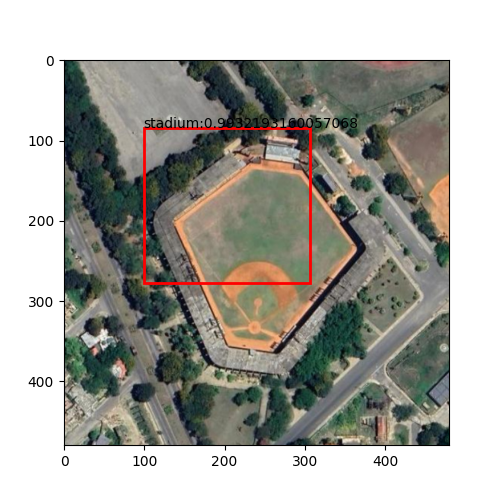
\includegraphics[width=0.5\textwidth]{Figure_1.png}
  \caption{Predicci\'on de Faster-RCNN}
  \label{fig:Figure_1}
\end{figure}

\begin{figure}[h]
  \centering
  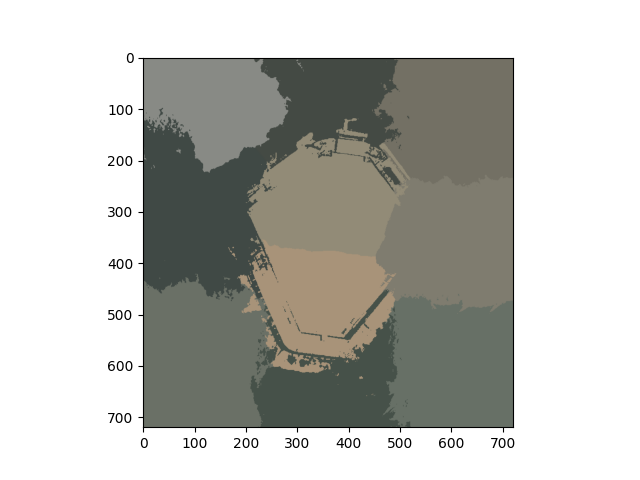
\includegraphics[width=0.5\textwidth]{Figure_2.png}
  \caption{K-Means RGB + XY}
  \label{fig:Figure_2}
\end{figure}

\begin{figure}[h]
  \centering
  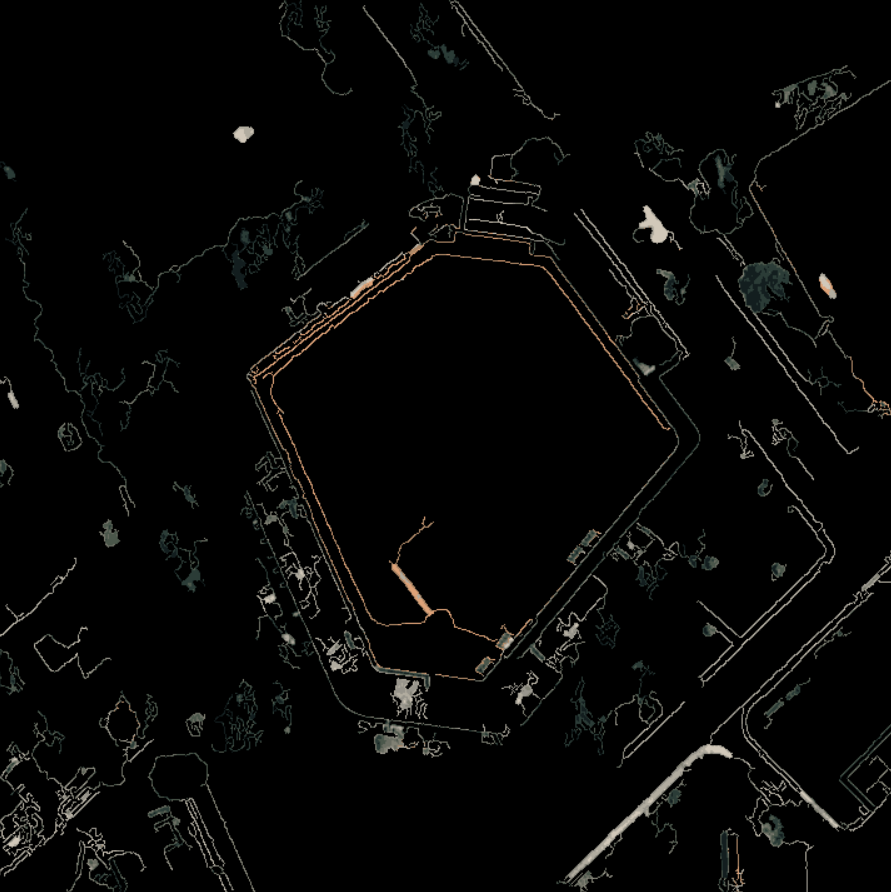
\includegraphics[width=0.5\textwidth]{canny.png}
  \caption{K-Means + Canny}
  \label{fig:canny}
\end{figure}

\begin{thebibliography}{8}
    \bibitem{citekey}
        K. He et al., “Deep residual learning for image recognition,” arXiv 1512.03385, Dec 2015.
  
    \bibitem{citekey}
        G. Huang, “Dense connected convolutional neural networks,” IEEE Computer Society Conference on Computer Vision and Pattern Recognition (CVPR), 2017.
    
    \bibitem{citekey}
        Ishii, Tomohiro, Edgar Simo-Serra, Satoshi Iizuka, Yoshihiko Mochizuki, Akihiro Sugimoto, Hiroshi Ishikawa, y Ryosuke Nakamura. «Detection by classification of buildings in multispectral satellite imagery». En 2016 23rd International Conference on Pattern Recognition (ICPR), 3344-49, 2016. https://doi.org/10.1109/ICPR.2016.7900150.
    
    \bibitem{citekey}
        Pritt, Mark, y Gary Chern. «Satellite Image Classification with Deep Learning». En 2017 IEEE Applied Imagery Pattern Recognition Workshop (AIPR), 1-7, 2017. https://doi.org/10.1109/AIPR.2017.8457969.

    \bibitem{citekey}
        Reda, Kinga, y Michal Kedzierski. «Detection, Classification and Boundary Regularization of Buildings in Satellite Imagery Using Faster Edge Region Convolutional Neural Networks». Remote Sensing 12, n.º 14 (enero de 2020): 2240. https://doi.org/10.3390/rs12142240.

    \bibitem{citekey}
        Christian Szegedy, Wei Liu, Yangqing Jia, Pierre Sermanet, Scott Reed, Dragomir Anguelov, Dumitru Erhan, Vincent Vanhoucke, and Andrew Rabinovich. "Going Deeper with Convolutions." Proceedings of the IEEE Conference on Computer Vision and Pattern Recognition (CVPR), 2015. doi: 10.1109/CVPR.2015.7298594

    \bibitem{citekey}
        François Chollet. "Xception: Deep Learning with Depthwise Separable Convolutions." Proceedings of the IEEE Conference on Computer Vision and Pattern Recognition (CVPR), 2017. doi: 10.1109/CVPR.2017.195

    \bibitem{citekey}
        W. Shao, "Unsupervised feature learning for urban land use classification using deep convolutional neural networks", ISPRS Journal of Photogrammetry and Remote Sensing, 2016
  \end{thebibliography}

\end{document}